% Upper-case Roman appendix numbering as required by section 1.6.
\chapter{Detailed Design Information}\label{app:design}
\section*{Pre-registered protocol (summary)}
Protocol v2 (\texttt{docs/paper/PROTOCOL\_V2.md}, committed 19 October 2026) fixes: the arms and their parity rules (identical folds, sampler, class balancing, label smoothing, augmentation, batch, epochs, schedule, last-epoch weights; only the backbone, input size, normalisation and learning-rate recipe may differ); the units per source; the selection rule (cross-validation pooled out-of-fold image QWK on the 5-class map); the primary endpoint (locked eye-level QWK, A$-$C, paired infant-clustered bootstrap, 2{,}000 replicates); Holm-corrected secondaries; descriptive endpoints; the minimum detectable difference ($\approx$0.08 eye QWK); the duplicate exclusion; and the conditions of the second locked opening. Its five amendments, each dated and committed before the experiment it governs, are:
\begin{enumerate}
\item[1.] (21 Oct) temperature fitted on eye-level driving-photograph vectors; the any-ROP threshold pooled over units and fitted on uncalibrated probabilities; headline numbers pooled over all prediction lists with one clustered interval; probe kernels' development predictions never opened.
\item[2.] (21 Oct) the learning rates chosen by the probe ($2\times10^{-4}$ for A, $10^{-4}$ for B, rule: keep $10^{-4}$ unless beaten by more than 0.03 macro-F1); disclosure that the probes ran before the duplicate exclusion was wired in; one kernel per arm and seed.
\item[3.] (22 Oct, after the A--E results) ensemble arm E; the cross-fitted ordinal decoder; arm D with log-sum-exp pooling, $K=8$, $\tau=1$, on the cross-validation-selected encoder.
\item[4.] (25 Oct, after the A--E results) arm G at 518~px; arm F with self-ensembling (EMA teacher 0.99, confidence 0.90, weight 1.0 ramped over two epochs) on the development half's photographs without labels, its development numbers marked transductive.
\item[5.] (31 Oct, after the A--G results, before any v4 run or locked scoring) the v4 round: (a) the data audit (near-duplicate sweep, Ostrava frame quality, cap re-ranking) applied to training rows only, with the folds, validation rows and exclusions unchanged, and two new leave-one-source-out folds (Ostrava, ROP-VL) beside the Shenzhen site fold; (b) models H (B on the v4 pool) and I (H plus the v4 recipe: EMA 0.999, one-epoch head warm-up, rotation $\pm180^\circ$, crop 0.85--1, gamma and noise, Fourier amplitude swap, label smoothing 0.10), and B on the two new LOSO folds; (c) the adoption rule of Equation~\ref{eq:adopt}, with H$-$B, I$-$B and I$-$H added to the paired contrasts and the locked half to be opened once for A--I together; (d) a budget of about 20 GPU-hours. A dated revision, written after the audit and before the pool, replaced the hospital-derived quality thresholds by per-camera thresholds without a field-of-view rule and required a pixel check for near-duplicates; a dated pre-run note, written before any v4 kernel, disclosed the zero weight for a class absent from a fold, the Fourier swap's handling of the zero-frequency term, the cap ranking and the EMA's start.
\end{enumerate}
\section*{Training configuration of model B}
Model: \texttt{vit\_small\_patch14\_reg4\_dinov2.lvd142m}, input 392~px, average pooling, dropout 0.3, drop-path 0.1, 6 outputs. Preprocessing: circle-crop, letterbox, CLAHE, ImageNet normalisation. Training: 20 epochs, batch 16, AdamW, peak learning rate $10^{-4}$, layer decay 0.8, weight decay 0.05, label smoothing 0.05, class-balanced weights ($\beta=0.999$), one-cycle cosine schedule (10\% warm-up), gradient clipping 1.0, mixed precision, strong augmentation (affine, perspective, blur, random erasing) and site randomisation (hue jitter, random greyscale, resolution jitter, random resized crop), no weighted sampler, no early stopping. Model~A differs in weights (RETFound-Green), normalisation (0.5/0.5) and peak learning rate ($2\times10^{-4}$); D adds the examination loss; F adds the adaptation block; G sets the input to 518~px; H reads the v4 fold files; I reads the v4 fold files and adds the recipe of Section~\ref{sec:v4design} (label smoothing 0.10, EMA decay 0.999, head warm-up 1 epoch, rotation 180, minimum crop scale 0.85, gamma 0.7--1.4 with $p=0.5$, noise $\sigma=0.02$ with $p=0.3$, Fourier block 3 with $p=0.5$).

\chapter{Raw Test Records and Supporting Data}\label{app:tests}
\section*{Per-fold cross-validation QWK (5-class), both seeds}
\begingroup\TightTable\small
\begin{tabularx}{\textwidth}{@{}p{30mm}YYYYY|YYYYY@{}}\toprule
 & \multicolumn{5}{c|}{Seed 42: folds 0--4} & \multicolumn{5}{c}{Seed 1337: folds 0--4}\\\midrule
A RETFound-Green & 0.62 & 0.87 & 0.87 & 0.91 & 0.92 & 0.59 & 0.87 & 0.88 & 0.91 & 0.92\\
B DINOv2 & 0.74 & 0.87 & 0.85 & 0.90 & 0.90 & 0.67 & 0.88 & 0.86 & 0.92 & 0.91\\
C EfficientNet (baseline) & 0.68 & 0.86 & 0.89 & 0.90 & 0.93 & 0.67 & 0.86 & 0.85 & 0.93 & 0.92\\
D DINOv2 + exam loss & 0.69 & 0.85 & 0.81 & 0.90 & 0.88 & 0.65 & 0.86 & 0.82 & 0.92 & 0.88\\
E Ensemble A+B+C & 0.68 & 0.87 & 0.91 & 0.92 & 0.93 & 0.63 & 0.88 & 0.88 & 0.93 & 0.94\\
F DINOv2 + adaptation & 0.67 & 0.89 & 0.84 & 0.93 & 0.88 & 0.65 & 0.89 & 0.88 & 0.91 & 0.91\\
G DINOv2 at 518 px & 0.67 & 0.88 & 0.88 & 0.92 & 0.89 & 0.65 & 0.88 & 0.88 & 0.92 & 0.92\\
H DINOv2, v4 pool & 0.66 & 0.88 & 0.83 & 0.92 & 0.91 & 0.67 & 0.88 & 0.84 & 0.91 & 0.91\\
I DINOv2, v4 pool + recipe & 0.68 & 0.88 & 0.87 & 0.91 & 0.91 & 0.70 & 0.88 & 0.82 & 0.92 & 0.89\\
\bottomrule
\end{tabularx}\endgroup
\par\small Generated by \url{scripts/rop_v3_report_tables.py} from \url{results/rop/v3/report_data.json}; duplicates excluded; Figure~\ref{fig:folds} draws the exact values.
\section*{Baseline confusion matrices}
\begin{figure}[htbp]
\centering
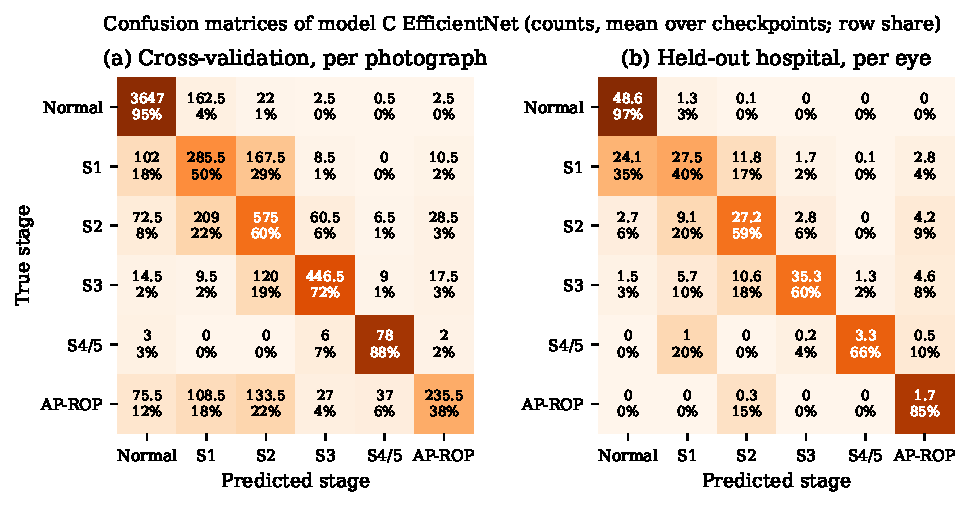
\includegraphics[width=\textwidth]{fig_confusion_C.pdf}
\caption{Confusion matrices of the EfficientNet baseline (model C)}\label{fig:confusionC}
\end{figure}
\begin{figure}[htbp]
\centering
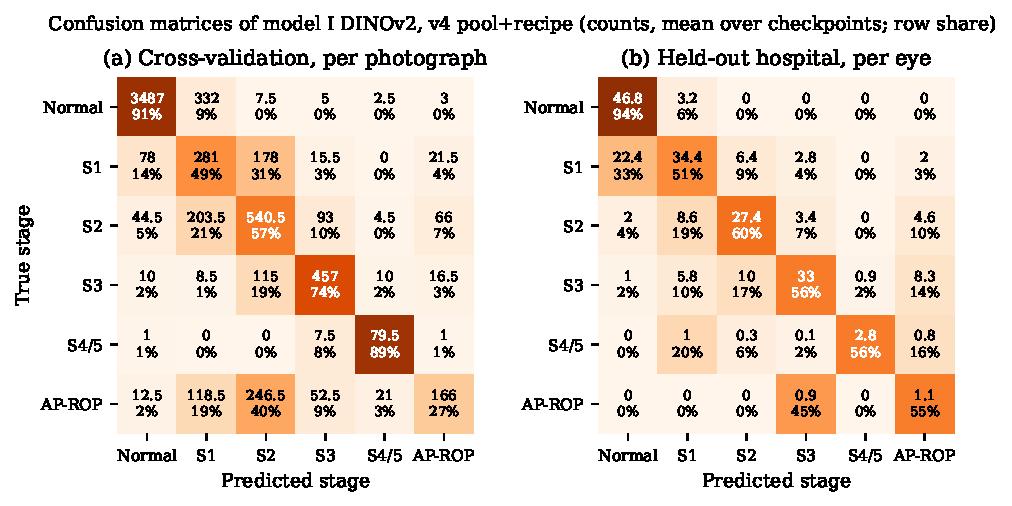
\includegraphics[width=\textwidth]{fig_confusion_I.pdf}
\caption{Confusion matrices of model I (v4 pool and recipe)}\label{fig:confusionI}
\end{figure}
\section*{Learning-rate probe}
Inner patient-disjoint split of fold~0's training rows (497 inner-validation photographs), seed 42, 20 epochs, macro-F1 at $3\times10^{-5}$ / $10^{-4}$ / $2\times10^{-4}$: RETFound-Green 0.717 / 0.755 / 0.812; DINOv2 0.747 / 0.764 / 0.772. Record: \texttt{results/rop/v3/lr\_probe.json}.
\section*{Cache gate}
Fold-0 baseline checkpoint scored on fold-0 validation from the cache and from the originals: argmax agreement 0.9917, $\Delta$QWK $-0.0006$, PSNR 52.85~dB over 200 images; 7{,}363 images cached, none missing. Record: \texttt{results/rop/v3/cache\_gate.json}.
\section*{Kaggle sessions}
Fourteen main sessions in v3 (A, B, D: one kernel each per seed; F, G: two kernels each per seed) and ten in v4 (B: one LOSO kernel per seed; H, I: two kernels each per seed, five CV folds and the site plus two LOSO folds), seven probe kernels and smoke runs, all on Tesla T4, all private. The v4 run log (\url{docs/v4/V4_RUN_LOG.md}) lists every arm, seed, fold and epoch. Kernel logs with per-epoch loss, learning rates, throughput, peak memory and (for F) the confidence mask rate are kept with the downloaded outputs.

\chapter{Software and Reproducibility Information}\label{app:software}
Repository: private GitHub repository \texttt{Coldbari/archive}, branch \texttt{v3-rop}; the results in this report are at commit \texttt{3f7b79f} (scores and report data \texttt{b827cce}; v3 runs \texttt{2620ba2}; v4 runs \texttt{e490423}, \texttt{5527d74}, \texttt{7b259be}; v4 model report \texttt{docs/v4/V4\_MODEL\_REPORT.md}). Dependencies: Python 3.14, PyTorch, timm, scikit-learn, pandas, NumPy, Pillow, OpenCV, Flask, ReportLab, matplotlib; pinned in the repository's requirements. To reproduce the numbers in this report without a GPU:
\begin{verbatim}
python scripts/rop_v3_score.py --v3     # -> results/rop/v3/v3_scores.json
python scripts/rop_v3_report_data.py    # -> results/rop/v3/report_data.json
python scripts/rop_v3_figures.py        # -> docs/report/figures/*.pdf
python scripts/rop_v3_report_tables.py  # -> tables/*.tex (incl. served model)
python -m pytest -q                     # 407 tests
\end{verbatim}
To retrain an arm: \url{python scripts/build_rop_cache.py}, then \url{python scripts/push_v3_kernels.py --arch dinov2_s --seed 42}, then \url{python scripts/collect_v3_run.py kaggle_cache/v3/<kernel>}. The eye-level route is \texttt{POST /predict\_eye} with fields \texttt{photos[]}, \texttt{eye} and \texttt{context}. The complete code is supplied as a digital attachment; the key modules are \url{models/common/architectures.py}, \url{optim.py}, \url{bag_loss.py}, \url{uda.py}, \url{units.py}, \url{v3_launch.py}, \url{scripts/rop_v3_score.py}, \url{webapp/inference.py} and \url{kaggle_kernels/rop_v3_finetune.py}.

\chapter{Project Management and Supporting Records}\label{app:management}
\section*{Plan and execution}
The work after the post-proposal review was planned as twelve tasks in a written implementation plan (19 October 2026), reviewed by a four-member panel of reviewer roles (lead, trainer, methodologist, critic) whose written reviews are kept with the plan. Each task was executed with a written brief, an implementer, a code review with findings, a fix round and a ledger entry; the ledger records every ruling and its cost if wrong. Four further rounds (ensemble and decoder; arm~D; arms~F and G; the v4 data audit with arms~H and I) followed the same process. Dates: protocol 19--21 October; training 21--27 October; scoring 27 October; v4 amendment, audit and pool 31 October; v4 training and scoring 31 October--1 November.
\section*{Individual contributions}
\FILL{12}{for each student, the subsystems, experiments and report sections they were responsible for}
\section*{Guide meetings and review actions}
\FILL{13}{from the log-book: dated guide meetings, the post-proposal review feedback and its closure, the request for approval of the locked-half scoring}
\section*{Outcome mapping}
\FILL{14}{programme-outcome mapping, if the department requires it}
